\DocumentMetadata{%
 %  uncompress, %only for debugging!!
  pdfversion=2.0,
  testphase={phase-II, tabular, graphic}%
 % testphase={phase-II,math, tabular, graphic}% TOC Does not work
   % testphase={phase-III,math}% TOC works
}
\tagpdfsetup{activate, tabsorder=structure}
% Use the following to fix bug in November 2023 download of LaTeX
\ExplSyntaxOn
\cs_generate_variant:Nn\__tag_prop_gput:Nnn{cnx}
\ExplSyntaxOff
\documentclass[11pt,
  english,
  letterpaper,
]{article}
\usepackage{sa4ss}
\usepackage{amsmath,amssymb,array}
\usepackage{booktabs}

% From tagged-template.latex
\usepackage{lmodern}
\usepackage{ifxetex,ifluatex}
\ifnum 0\ifxetex 1\fi\ifluatex 1\fi=0 % if pdftex
  \usepackage[T1]{fontenc}
  \usepackage[utf8]{inputenc}
  \usepackage{textcomp} % provide euro and other symbols
\else % if luatex or xetex
  \usepackage{unicode-math}
  \defaultfontfeatures{Scale=MatchLowercase}
  \defaultfontfeatures[\rmfamily]{Ligatures=TeX,Scale=1}
\fi

% Use upquote if available, for straight quotes in verbatim environments
\IfFileExists{upquote.sty}{\usepackage{upquote}}{}
\IfFileExists{microtype.sty}{% use microtype if available
  \usepackage[]{microtype}
  \UseMicrotypeSet[protrusion]{basicmath} % disable protrusion for tt fonts
}{}
\makeatletter
\@ifundefined{KOMAClassName}{% if non-KOMA class
  \IfFileExists{parskip.sty}{%
    \usepackage{parskip}
  }{% else
    \setlength{\parindent}{0pt}
    \setlength{\parskip}{6pt plus 2pt minus 1pt}}
}{% if KOMA class
  \KOMAoptions{parskip=half}}
\makeatother
\usepackage{xcolor}
\IfFileExists{xurl.sty}{\usepackage{xurl}}{} % add URL line breaks if available
\hypersetup{
  pdftitle={Status of Copper Rockfish (Sebastes caurinus) along the California North of Pt. Conception U.S. West coast in 2022},
  pdflang={en},
  hidelinks,
  pdfcreator={LaTeX via pandoc}}
\urlstyle{same} % disable monospaced font for URLs
\usepackage{longtable}
% Correct order of tables after \paragraph or \subparagraph
\usepackage{etoolbox}
\makeatletter
\patchcmd\longtable{\par}{\if@noskipsec\mbox{}\fi\par}{}{}
\makeatother
% Allow footnotes in longtable head/foot
\IfFileExists{footnotehyper.sty}{\usepackage{footnotehyper}}{\usepackage{footnote}}
\makesavenoteenv{longtable}
\usepackage{graphicx}
\makeatletter
\def\maxwidth{\ifdim\Gin@nat@width>\linewidth\linewidth\else\Gin@nat@width\fi}
\def\maxheight{\ifdim\Gin@nat@height>\textheight\textheight\else\Gin@nat@height\fi}
\makeatother
% Scale images if necessary, so that they will not overflow the page
% margins by default, and it is still possible to overwrite the defaults
% using explicit options in \includegraphics[width, height, ...]{}
\setkeys{Gin}{width=\maxwidth,height=\maxheight,keepaspectratio}
% Set default figure placement to htbp
\makeatletter
\def\fps@figure{htbp}
\makeatother
\setlength{\emergencystretch}{3em} % prevent overfull lines
\providecommand{\tightlist}{%
  \setlength{\itemsep}{0pt}\setlength{\parskip}{0pt}}
\setcounter{secnumdepth}{5}
\ifxetex
  % Load polyglossia as late as possible: uses bidi with RTL langages (e.g. Hebrew, Arabic)
  \usepackage{polyglossia}
  \setmainlanguage[]{english}
\else
  \usepackage[shorthands=off,main=english]{babel}
\fi

%Define cslreferences environment, required by pandoc 2.8
%https://github.com/rstudio/rmarkdown/issues/1649
\newlength{\csllabelwidth}
\setlength{\csllabelwidth}{3em}
\newlength{\cslhangindent}
\setlength{\cslhangindent}{1.5em}
% for Pandoc 2.8 to 2.10.1
\newenvironment{cslreferences}%
  {}%
  {\par}
% For Pandoc 2.11+
\newenvironment{CSLReferences}[2] % #1 hanging-ident, #2 entry spacing
 {% don't indent paragraphs
  \setlength{\parindent}{0pt}
  % turn on hanging indent if param 1 is 1
  \ifodd #1 \everypar{\setlength{\hangindent}{\cslhangindent}}\ignorespaces\fi
  % set entry spacing
  \ifnum #2 > 0
  \setlength{\parskip}{#2\baselineskip}
  \fi
 }%
 {}
\usepackage{calc}  % for \widthof, \maxof in minipage
\newcommand{\CSLBlock}[1]{#1\hfill\break}
\newcommand{\CSLLeftMargin}[1]{\parbox[t]{\csllabelwidth}{#1}}
\newcommand{\CSLRightInline}[1]{\parbox[t]{\linewidth - \csllabelwidth}{#1}\break}
\newcommand{\CSLIndent}[1]{\hspace{\cslhangindent}#1}


\providecommand{\tightlist}{%
  \setlength{\itemsep}{0pt}\setlength{\parskip}{0pt}}


\date{}
\newcommand{\trTitle}{Status of Copper Rockfish (\emph{Sebastes caurinus}) along the California North of Pt. Conception U.S. West coast in 2022}
\newcommand{\trYear}{2022}
\newcommand{\trMonth}{December}
\newcommand{\trAuthsLong}{truetruetrue}
\newcommand{\trAuthsBack}{Monk, M.H., C.R. Wetzel, J. Coates}
\newcommand{\trCitation}{
\begin{hangparas}{1em}{1}
\trAuthsBack{}. \trYear{}. \trTitle{}. \glsentrylong{pfmc}, Portland, Oregon. \pageref{LastPage}{}\,p.
\end{hangparas}}

\begin{document}

%%%%% Frontmatter %%%%%

% Footnote symbols in front matter
\renewcommand*{\thefootnote}{\fnsymbol{footnote}}

\small
\thispagestyle{empty}
\pagenumbering{roman}
\noindent
\begin{center}
\title{Status of Copper Rockfish (\emph{Sebastes caurinus}) along the California North of Pt. Conception U.S. West coast in 2022}
% \textnormal{\MakeTextUppercase{\trTitle{}}}
\vspace{1.5cm}
{\Large\textbf\newline{Status of Copper Rockfish (\emph{Sebastes caurinus}) along the California North of Pt. Conception U.S. West coast in 2022}}
\vfill
by\\
Melissa H. Monk\textsuperscript{1}\\
Chantel R. Wetzel\textsuperscript{2}\\
Julia Coates\textsuperscript{3}\vfill
\textsuperscript{1}Southwest Fisheries Science Center, U.S. Department of Commerce, National Oceanic and Atmospheric Administration, National Marine Fisheries Service, 110 McAllister Way, Santa Cruz, California 95060\\
\textsuperscript{2}Northwest Fisheries Science Center, U.S. Department of Commerce, National Oceanic and Atmospheric Administration, National Marine Fisheries Service, 2725 Montlake Boulevard East, Seattle, Washington 98112\\
\textsuperscript{3}.na.character\vfill
\trMonth{} \trYear{}
\end{center}
\clearpage

% Fourth page: Colophon
\thispagestyle{empty}
\vspace*{\fill}
\begin{center}
\copyright{} \glsentrylong{pfmc}, \trYear{}\\
\end{center}
\par
\bigskip
\noindent
Correct citation for this publication:
\bigskip
\par
\trCitation{}
\clearpage

% Add TOC to pdf bookmarks (clickable pdf)
\pdfbookmark[1]{\contentsname}{toc}

% Table of contents page, lists of figures and tables
\tableofcontents\clearpage
\label{TRlastRoman}
\clearpage

% Table of contents
\newpage
\thispagestyle{empty} % to remove page number

% Settings for the main document
\pagenumbering{arabic}  % Regular page numbers
\pagestyle{plain}  % No page number on first page of main document, use 'empty'
\renewcommand*{\thefootnote}{\arabic{footnote}}  % Back to numeric footnotes
\setcounter{footnote}{0}  % And start at 1
\renewcommand{\headrulewidth}{0.5pt}
\renewcommand{\footrulewidth}{0.5pt}
%\pagestyle{fancy}\fancyhead[c]{Draft: Do not cite or circulate}

\newcommand{\lt}{\ensuremath <}
\newcommand{\gt}{\ensuremath >}

\pagebreak
\pagenumbering{roman}
\setcounter{page}{1}

\renewcommand{\thetable}{\roman{table}}
\renewcommand{\thefigure}{\roman{figure}}

\setlength\parskip{0.5em plus 0.1em minus 0.2em}

\hypertarget{executive-summary}{%
\section*{Executive summary}\label{executive-summary}}
\addcontentsline{toc}{section}{Executive summary}

\hypertarget{stock}{%
\subsection*{Stock}\label{stock}}
\addcontentsline{toc}{subsection}{Stock}

This assessment reports the status of copper rockfish (\emph{Sebastes caurinus}) off the California North of Pt. Conception U.S. West coast using data through xxxx.

\hypertarget{catches}{%
\subsection*{Catches}\label{catches}}
\addcontentsline{toc}{subsection}{Catches}

Replace text with trends and current levels. Include Table for last 10 years. Include Figure with long-term estimates.

\hypertarget{data-and-assessment}{%
\subsection*{Data and assessment}\label{data-and-assessment}}
\addcontentsline{toc}{subsection}{Data and assessment}

This assessment uses the stock assessment framework Stock Synthesis

(SS3).

Replace text with date of last assessment, type of assessment model, data available, new information, and information lacking.

\hypertarget{stock-biomass-and-dynamics}{%
\subsection*{Stock biomass and dynamics}\label{stock-biomass-and-dynamics}}
\addcontentsline{toc}{subsection}{Stock biomass and dynamics}

Replace text with trends and current levels relative to virgin or historic levels and description of uncertainty. Include Table for last 10 years. Include Figure with long-term estimates.

\hypertarget{recruitment}{%
\subsection*{Recruitment}\label{recruitment}}
\addcontentsline{toc}{subsection}{Recruitment}

Replace text with trends and current levels relative to virgin or historic levels and description of uncertainty. Include Table for last 10 years. Include Figure with long-term estimates.

\hypertarget{exploitation-status}{%
\subsection*{Exploitation status}\label{exploitation-status}}
\addcontentsline{toc}{subsection}{Exploitation status}

Replace text with total catch divided by exploitable biomass or SPR harvest rate. Include Table for last 10 years. Include Figure with trend in f relative to target vs.~trend in biomass relative to the target.

\hypertarget{ecosystem-considerations}{%
\subsection*{Ecosystem considerations}\label{ecosystem-considerations}}
\addcontentsline{toc}{subsection}{Ecosystem considerations}

Replace text with a summary of reviewed environmental and ecosystem factors that appear to be correlated with stock dynamics. These may include variability in they physical environment, habitat, competitors, prey, or predators that directly or indirectly affects the stock's status, vital rates (growth, survival, productivity/recruitment) or range and distribution. Note which, if any, ecosystem factors are used in the assessment and how (e.g., as background information, in data preparations, as data inputs, in decisions about model structure).

\hypertarget{reference-points}\), i.e., the \(B_{MSY}\) proxy and the equilibrium stock size that results from fishing at the default harvest rate, i.e., the \(F_{MSY}\) proxy. Include Table of estimated reference points for ssb, SPR, exploitation rate, and yield based on SSB proxy for MSY, SPR proxy for MSY, and estimated MSY values.

\hypertarget{management-performance}{%
\subsection*{Management performance}\label{management-performance}}
\addcontentsline{toc}{subsection}{Management performance}

Include Table of most recent 10 years of catches in comparison with OFL, ABC, HG, and OY/ACL values, overfishing levels, actual catch and discard. Include OFL (encountered), OFL (retained), and OFL (dead) if different due to discard and discard mortality.

\hypertarget{unresolved-problems-and-major-uncertainties}{%
\subsection*{Unresolved problems and major uncertainties}\label{unresolved-problems-and-major-uncertainties}}
\addcontentsline{toc}{subsection}{Unresolved problems and major uncertainties}

Replace text with any special issues that complicate scientific assessment, questions about the best model scenario, etc.

\hypertarget{decision-table-and-projections}{%
\subsection*{Decision table and projections}\label{decision-table-and-projections}}
\addcontentsline{toc}{subsection}{Decision table and projections}

Replace text with projected yields (OFL, ABC, and ACL), spawning biomass, and stock depletion levels for each year. OFL calculations should be based on the assumption that future catches equal ABCs and not OFLs.

\hypertarget{scientific-uncertainty}{%
\subsection*{Scientific uncertainty}\label{scientific-uncertainty}}
\addcontentsline{toc}{subsection}{Scientific uncertainty}

Replace text with the sigma value and the basis for its calculation.

\hypertarget{research-and-data-needs}{%
\subsection*{Research and data needs}\label{research-and-data-needs}}
\addcontentsline{toc}{subsection}{Research and data needs}

Replace text with information gaps that seriously impede the stock assessment.

\pagebreak
\setlength{\parskip}{5mm plus1mm minus1mm}
\pagenumbering{arabic}
\setcounter{page}{1}
\renewcommand{\thefigure}{\arabic{figure}}
\renewcommand{\thetable}{\arabic{table}}
\setcounter{table}{0}
\setcounter{figure}{0}

\hypertarget{introduction}{%
\section{Introduction}\label{introduction}}

\hypertarget{basic-information}{%
\subsection{Basic Information}\label{basic-information}}

This assessment reports the status of copper rockfish (\emph{Sebastes caurinus}) off the California coast, north of Point Conception, using data through 2022.

Copper rockfish is a medium- to large-sized nearshore rockfish found from Mexico to Alaska. The core range is comparatively large, from northern Baja Mexico to the Gulf of Alaska, as well as in Puget Sound. Copper rockfish have historically been a part of both commercial and recreational fisheries throughout its range.

Copper rockfish are commonly found in waters less than 130 meters in depth in nearshore kelp forests and rocky habitat (Love 1996). The diets of copper rockfish consist primarily of crustaceans, mollusks, and fish (Lea, McAllister, and VenTresca 1999; Bizzarro, Yoklavich, and Wakefield 2017). The body coloring of copper rockfish varies across the West Coast with northern fish often exhibiting dark brown to olive with southern fish exhibiting yellow to olive-pink variations in color (D. J. Miller and Lea 1972), which initially led to them being designated as two separate species (\emph{S. caurinus} and \emph{S. vexillaris}).

Numerous genetic studies have been performed looking for genetic variation in copper rockfish, with variable outcomes. Genetic work has revealed significant differences between Puget Sound and coastal stocks (Dick, Shurin, and Taylor 2014). Stocks along the West Coast have not been determined to be genetically distinct populations, but significant population subdivision has been detected, indicating limited oceanographic exchange among geographically proximate locations (Buonaccorsi et al. 2002; Johansson et al. 2008). A specific study examining copper rockfish populations off the coast of Santa Barbara and Monterey California identified a genetic break between the north and south, with moderate differentiation (Sivasundar and Palumbi 2010).

Copper rockfish are a relatively long-lived rockfish, estimated to live at least 50 years (Love 1996). Copper rockfish was determined to have the highest vulnerability (V = 2.27) of any West Coast groundfish stock evaluated in a productivity susceptibility analysis (Cope et al. 2011). This analysis calculated species-specific vulnerability scores based on two dimensions: productivity characterized by the life history and susceptibility that characterized how the stock could be impacted by fisheries and other activities.

\hypertarget{life-history}{%
\subsection{Life History}\label{life-history}}

Replace text.

\hypertarget{ecosystem-considerations-1}{%
\subsection{Ecosystem Considerations}\label{ecosystem-considerations-1}}

Replace text.

\hypertarget{historical-and-current-fishery-information}{%
\subsection{Historical and Current Fishery Information}\label{historical-and-current-fishery-information}}

Off the coast of California, north of Point Conception, copper rockfish is caught in both commercial and recreational fisheries. Recreational removals have been the largest source of fishing mortality, comprising nearly 85 percent of total removals of copper rockfish across all years (Table XX and Figure XX). The landings from the commercial fishery have been minimal by year, expect for a brief period between the mid-1980s and early-2000s.

The recreational fishery in the early part of the 20th century was focused on nearshore waters near ports, with expanded activity further from port and into deeper depths over time (R. R. Miller et al. 2014). Prior to the groundfish fishery being declared a federal disaster in 2000, and the subsequent rebuilding period, there were no time or area closures for groundfish. Access to deeper depths during this period spread effort over a larger area and filled bag limits with a greater diversity of species from both the shelf and nearshore. This resulted in lower catch of nearshore rockfish relative to the period after 2000 when 20 to 60 fm depth restrictions ranging from 20 fm in the Northern Management Area to 60 fm in the Southern Management Area were put in place in various management area delineations along the state (see Appendix Section \ref{ca-man}). This shifting effort onto the nearshore, concomitantly increased catch rates for nearshore rockfish including copper rockfish in the remaining open depths, though season lengths were greatly curtailed.

Following all previously overfished groundfish species, other than yelloweye rockfish, being declared rebuilt by 2019, deeper depth restrictions were offered in the Southern Management area allowing resumed access to shelf rockfish in less than 75 fm and are currently 100 fm as of 2021. The increased access to deeper depths south of Point Conception with the rebuilding of cowcod is expected to reduce the effort in nearshore waters where copper rockfish is most prevalent. To the north of Point Conception where yelloweye rockfish are prevalent, depth constraints persist and effort remains focused on the nearshore in 30 to 50 fm depending on the management area. As yelloweye rockfish continues to rebuild, incremental increases in access to deeper depths are expected, which will likely further reduce the effort in nearshore waters where copper rockfish is most prevalent.

Prior to development of the live fish market in the 1980s, there was very little commercial catch of copper rockfish, with dead copper rockfish fetching a low ex-vessel price per pound. Copper rockfish were targeted along with other rockfish to some degree in the nearshore or caught as incidental catch by vessels targeting other more valuable stocks such as lingcod. Most fish were caught using hook and line gear, though some were caught using traps, gill nets and, rarely, trawl gear. Trawling was prohibited within three miles of shore in 1953 and gill netting within three miles of shore was prohibited in 1994, preventing access to a high proportion of the species habitat with these gear types. Copper rockfish were caught along with other rockfish to some degree in the nearshore or caught as bycatch by vessels targeting other more valuable stocks such as lingcod.

In the late 1980s and early 1990s a market for fish landed live arose out of Los Angeles and the Bay area, driven by demand from Asian restaurants and markets. The growth of the live fish market was driven by consumers willing to pay a higher price for live fish, ideally plate-sized (12 - 14 inches or 30.5 - 35.6 cm). Live fish landed for the restaurant market are lumped into two categories, small (1 - 3 lbs.) or large (3 - 6 lbs.), with small, plate-sized, fish fetching higher prices at market ranging between \$5 -7 per fish (Bill James, personal communication). Copper rockfish is one of the many rockfish species that is included in the commercial live fish fishery. The proportion of copper rockfish being landed live vs.~dead since 2000 by California commercial fleets ranges between 50 to greater than 70 percent in the southern and northern areas, respectively.

With the development and expansion of the nearshore live fish fishery during the 1980s and 1990s, new entrants in this open access fishery were drawn by premium ex-vessel price per pound for live fish, resulting in over-capitalization of the fishery. Since 2002, the California Department of Fish and Wildlife (CDFW) has managed 19 nearshore species in accordance with Nearshore Fisheries Management Plan (Wilson-Vandenberg, Larinto, and Key 2014). In 2003, the CDFW implemented a Nearshore Restricted Access Permit system, including the requirement of a Deeper Nearshore Fishery Species Permit to retain copper rockfish, with the overall goal of reducing the number of participants to a more sustainable level, with permit issuance based on historical landings history by the retrospective qualifying date. The result was a reduction in permits issued from 1,127 in 1999 to 505 in 2003, greatly reducing catch levels. In addition, reduced trip limits, season closures in March and April and depth restrictions were implemented to address bycatch of overfished species and associated constraints from their low catch limits.

Copper rockfish residing between Point Conception and the California/Oregon border are assessed here as a single, separate stock (Figure \ref{fig:map}). This designation was made based on oceanographic, geographic, and fishery conditions. The copper rockfish population in California waters was split at Point Conception due to water circulation patterns that create a natural barrier between nearshore rockfish populations to the north and south. The northern border for this assessment was defined as the California/Oregon border due to substantial differences in historical and current exploitation levels. Additionally, the fairly sedentary nature of adult copper rockfish, likely limits flow of fish between northern California and areas to the north.

\hypertarget{summary-of-management-history-and-performance}{%
\subsection{Summary of Management History and Performance}\label{summary-of-management-history-and-performance}}

Replace text.

\hypertarget{foreign-fisheries}{%
\subsection{Foreign Fisheries}\label{foreign-fisheries}}

Replace text.

\hypertarget{data}{%
\section{Data}\label{data}}

Data comprise the foundational components of stock assessment models. The decision to include or exclude particular data sources in an assessment model depends on many factors. These factors often include, but are not limited to, the way in which data were collected (e.g., measurement method and consistency); the spatial and temporal coverage of the data; the quantity of data available per desired sampling unit; the representativeness of the data to inform the modeled processes of importance; timing of when the data were provided; limitations imposed by the Terms of Reference; and the presence of an avenue for the inclusion of the data in the assessment model. Attributes associated with a data source can change through time, as can the applicability of the data source when different modeling approaches are explored (e.g., stock structure or time-varying processes). Therefore, the specific data sources included or excluded from this assessment should not necessarily constrain the selection of data sources applicable to future stock assessments for copper rockfish. Even if a data source is not directly used in the stock assessment they can provide valuable insights into biology, fishery behavior, or localized dynamics.

Data from a wide range of programs were available for possible inclusion in the current assessment model. Descriptions of each data source included in the model (Figure \ref{fig:data-plot}) and sources that were explored but not included in the base model are provided below. Data that were excluded from the base model were explicitly explored during the development of this stock assessment or have not changed since their past exploration in a previous copper rockfish stock assessment. In some cases, the inclusion of excluded data sources were explored through sensitivity analyses (see Section \ref{assessment-model}).

\hypertarget{fishery-dependent-data}{%
\subsection{Fishery-Dependent Data}\label{fishery-dependent-data}}

\hypertarget{fishery-independent-data}{%
\subsection{Fishery-Independent Data}\label{fishery-independent-data}}

\hypertarget{section}{%
\subsubsection{\texorpdfstring{\acrlong{s-aslope}}{}}\label{section}}

The \gls{s-aslope} operated during the months of October to November aboard the R/V \emph{Miller Freeman}. Partial survey coverage of the US west coast occurred during the years 1988-1996 and complete coverage (north of 34\textdegree 30\textquotesingle S) during the years 1997 and 1999-2001. Typically, only these four years that are seen as complete surveys are included in assessments.

\hypertarget{section-1}{%
\subsubsection{\texorpdfstring{\acrlong{s-ccfrp}}{}}\label{section-1}}

Since 2007, the \gls{s-ccfrp} has monitored several areas in California to evaluate the performance of \glspl{mpa} and understand nearshore fish populations (Wendt and Starr 2009; Starr et al. 2015). In 2017, the survey expanded beyond the four \Gls{mpa}s in central California (Año Nuevo, Point Lobos, Point Buchon, and Piedras Blancas) to include the entire California coast. Fish are collected by volunteer anglers aboard \glspl{cpfv} guided by one of the following academic institutions based on proximity to fishing location: Humboldt State University; Bodega Marine Laboratories; Moss Landing Marine Laboratories; Cal Poly San Luis Obispo; University of California, Santa Barbara; and Scripps Institution of Oceanography.

Surveys consist of fishing with hook-and-line gear for 30-45 minutes within randomly chosen 500 by 500 m grid cells within and outside \glspl{mpa}. Prior to 2017, all fish were measured for length and release or descended to depth; since then, some were sampled for otoliths and fin clips.

\hypertarget{section-2}{%
\subsubsection{\texorpdfstring{\acrlong{s-tri}}{}}\label{section-2}}

The \gls{s-tri} was first conducted by the \gls{afsc} in 1977, and the survey continued until 2004 (Weinberg et al. 2002). Its basic design was a series of equally-spaced east-to-west transects across the continential shelf from which searches for tows in a specific depth range were initiated. The survey design changed slightly over time. In general, all of the surveys were conducted in the mid summer through early fall. The 1977 survey was conducted from early July through late September. The surveys from 1980 through 1989 were conducted from mid-July to late September. The 1992 survey was conducted from mid July through early October. The 1995 survey was conducted from early June through late August. The 1998 survey was conducted from early June through early August. Finally, the 2001 and 2004 surveys were conducted from May to July.

Haul depths ranged from 91-457 m during the 1977 survey with no hauls shallower than 91 m. Due to haul performance issues and truncated sampling with respect to depth, the data from 1977 were omitted from this analysis. The surveys in 1980, 1983, and 1986 covered the US West Coast south to 36.8\textdegree N latitude and a depth range of 55-366 m. The surveys in 1989 and 1992 covered the same depth range but extended the southern range to 34.5\textdegree N (near Point Conception). From 1995 through 2004, the surveys covered the depth range 55-500 m and surveyed south to 34.5\textdegree N. In 2004, the final year of the \gls{s-tri} series, the \gls{nwfsc} \gls{fram} conducted the survey following similar protocols to earlier years.

\hypertarget{section-3}{%
\subsubsection{\texorpdfstring{\acrlong{s-wcgbt}}{}}\label{section-3}}

The \Gls{s-wcgbt} is based on a random-grid design; covering the coastal waters from a depth of 55-1,280 m (Bradburn, Keller, and Horness 2011). This design generally uses four industry-chartered vessels per year assigned to a roughly equal number of randomly selected grid cells and divided into two `passes' of the coast. Two vessels fish from north to south during each pass between late May to early October. This design therefore incorporates both vessel-to-vessel differences in catchability, as well as variance associated with selecting a relatively small number (approximately 700) of possible cells from a very large set of possible cells spread from the Mexican to the Canadian borders.

\hypertarget{biological-data}{%
\subsection{Biological Data}\label{biological-data}}

\hypertarget{natural-mortality}{%
\subsubsection{Natural Mortality}\label{natural-mortality}}

\hypertarget{maturation-and-fecundity}{%
\subsubsection{Maturation and Fecundity}\label{maturation-and-fecundity}}

\hypertarget{sex-ratio}{%
\subsubsection{Sex Ratio}\label{sex-ratio}}

\hypertarget{length-weight-relationship}{%
\subsubsection{Length-Weight Relationship}\label{length-weight-relationship}}

\hypertarget{growth-length-at-age}{%
\subsubsection{Growth (Length-at-Age)}\label{growth-length-at-age}}

\hypertarget{ageing-precision-and-bias}{%
\subsubsection{Ageing Precision and Bias}\label{ageing-precision-and-bias}}

\hypertarget{environmental-and-ecosystem-data}{%
\subsection{Environmental and Ecosystem Data}\label{environmental-and-ecosystem-data}}

\hypertarget{assessment-model}{%
\section{Assessment Model}\label{assessment-model}}

\hypertarget{summary-of-previous-assessments-and-reviews}{%
\subsection{Summary of Previous Assessments and Reviews}\label{summary-of-previous-assessments-and-reviews}}

\hypertarget{history-of-modeling-approaches-not-required-for-an-update-assessment}{%
\subsubsection{History of Modeling Approaches (not required for an update assessment)}\label{history-of-modeling-approaches-not-required-for-an-update-assessment}}

\hypertarget{most-recent-star-panel-and-ssc-recommendations-not-required-for-an-update-assessment}{%
\subsubsection{Most Recent STAR Panel and SSC Recommendations (not required for an update assessment)}\label{most-recent-star-panel-and-ssc-recommendations-not-required-for-an-update-assessment}}

\hypertarget{response-to-groundfish-subcommittee-requests-not-required-in-draft}{%
\subsubsection{Response to Groundfish Subcommittee Requests (not required in draft)}\label{response-to-groundfish-subcommittee-requests-not-required-in-draft}}

\hypertarget{model-structure-and-assumptions}{%
\subsection{Model Structure and Assumptions}\label{model-structure-and-assumptions}}

\hypertarget{model-changes-from-the-last-assessment-not-required-for-an-update-assessment}{%
\subsubsection{Model Changes from the Last Assessment (not required for an update assessment)}\label{model-changes-from-the-last-assessment-not-required-for-an-update-assessment}}

\hypertarget{modeling-platform-and-structure}{%
\subsubsection{Modeling Platform and Structure}\label{modeling-platform-and-structure}}

General model specifications (e.g., executable version, model structure, definition of fleets and areas)

\hypertarget{model-parameters}{%
\subsubsection{Model Parameters}\label{model-parameters}}

Describe estimated vs.~fixed parameters, priors

\hypertarget{key-assumptions-and-structural-choices}{%
\subsubsection{Key Assumptions and Structural Choices}\label{key-assumptions-and-structural-choices}}

\hypertarget{base-model-results}{%
\subsection{Base Model Results}\label{base-model-results}}

\hypertarget{parameter-estimates}{%
\subsubsection{Parameter Estimates}\label{parameter-estimates}}

\hypertarget{fits-to-the-data}{%
\subsubsection{Fits to the Data}\label{fits-to-the-data}}

\hypertarget{population-trajectory}{%
\subsubsection{Population Trajectory}\label{population-trajectory}}

\hypertarget{reference-points-1}{%
\subsubsection{Reference Points}\label{reference-points-1}}

\hypertarget{model-diagnostics}{%
\subsection{Model Diagnostics}\label{model-diagnostics}}

Describe all diagnostics

\hypertarget{convergence}{%
\subsubsection{Convergence}\label{convergence}}

\hypertarget{sensitivity-analyses}{%
\subsubsection{Sensitivity Analyses}\label{sensitivity-analyses}}

\hypertarget{retrospective-analysis}{%
\subsubsection{Retrospective Analysis}\label{retrospective-analysis}}

\hypertarget{likelihood-profiles}{%
\subsubsection{Likelihood Profiles}\label{likelihood-profiles}}

\hypertarget{unresolved-problems-and-major-uncertainties-1}{%
\subsubsection{Unresolved Problems and Major Uncertainties}\label{unresolved-problems-and-major-uncertainties-1}}

\hypertarget{management}{%
\section{Management}\label{management}}

\hypertarget{reference-points-2}{%
\subsection{Reference Points}\label{reference-points-2}}

\hypertarget{unresolved-problems-and-major-uncertainties-2}{%
\subsection{Unresolved Problems and Major Uncertainties}\label{unresolved-problems-and-major-uncertainties-2}}

\hypertarget{harvest-projections-and-decision-tables}{%
\subsection{Harvest Projections and Decision Tables}\label{harvest-projections-and-decision-tables}}

\hypertarget{evaluation-of-scientific-uncertainty}{%
\subsection{Evaluation of Scientific Uncertainty}\label{evaluation-of-scientific-uncertainty}}

\hypertarget{research-and-data-needs-1}{%
\subsection{Research and Data Needs}\label{research-and-data-needs-1}}

\hypertarget{acknowledgments}{%
\section{Acknowledgments}\label{acknowledgments}}

Here are all the mad props!

\clearpage

\hypertarget{references}{%
\section{References}\label{references}}

\hypertarget{refs}{}
\begin{CSLReferences}{1}{0}
\leavevmode\vadjust pre{\hypertarget{ref-bizzarro_diet_2017-1}{}}%
Bizzarro, Joseph J., Mary M. Yoklavich, and W. Waldo Wakefield. 2017. {``Diet Composition and Foraging Ecology of {U}.{S}. {Pacific} {Coast} Groundfishes with Applications for Fisheries Management.''} \emph{Environmental Biology of Fishes} 100 (4): 375--93. \url{https://doi.org/10.1007/s10641-016-0529-2}.

\leavevmode\vadjust pre{\hypertarget{ref-bradburn_2003_2011}{}}%
Bradburn, M. J., A. A Keller, and B. H. Horness. 2011. {``The 2003 to 2008 {US} {West} {Coast} Bottom Trawl Surveys of Groundfish Resources Off {Washington}, {Oregon}, and {California}: Estimates of Distribution, Abundance, Length, and Age Composition.''} US Department of Commerce, National Oceanic; Atmospheric Administration, National Marine Fisheries Service.

\leavevmode\vadjust pre{\hypertarget{ref-buonaccorsi_population_2002}{}}%
Buonaccorsi, Vincent P, Carol A Kimbrell, Eric A Lynn, and Russell D Vetter. 2002. {``Population Structure of Copper Rockfish (\emph{{Sebastes} Caurinus}) Reflects Postglacial Colonization and Contemporary Patterns of Larval Dispersal.''} \emph{Canadian Journal of Fisheries and Aquatic Sciences} 59 (8): 1374--84. \url{https://doi.org/10.1139/f02-101}.

\leavevmode\vadjust pre{\hypertarget{ref-cope_approach_2011}{}}%
Cope, Jason M., John DeVore, E. J. Dick, Kelly Ames, John Budrick, Daniel L. Erickson, Joanna Grebel, et al. 2011. {``An {Approach} to {Defining} {Stock} {Complexes} for {U}.{S}. {West} {Coast} {Groundfishes} {Using} {Vulnerabilities} and {Ecological} {Distributions}.''} \emph{North American Journal of Fisheries Management} 31 (4): 589--604. \url{https://doi.org/10.1080/02755947.2011.591264}.

\leavevmode\vadjust pre{\hypertarget{ref-dick_replicate_2014}{}}%
Dick, S., J. B. Shurin, and E. B. Taylor. 2014. {``Replicate Divergence Between and Within Sounds in a Marine Fish: The Copper Rockfish ( \emph{{Sebastes} Caurinus} ).''} \emph{Molecular Ecology} 23 (3): 575--90. \url{https://doi.org/10.1111/mec.12630}.

\leavevmode\vadjust pre{\hypertarget{ref-johansson_influence_2008}{}}%
Johansson, M. L., M. A. Banks, K. D. Glunt, H. M. Hassel-Finnegan, and V. P. Buonaccorsi. 2008. {``Influence of Habitat Discontinuity, Geographical Distance, and Oceanography on Fine-Scale Population Genetic Structure of Copper Rockfish ( \emph{{Sebastes} Caurinus} ).''} \emph{Molecular Ecology} 17 (13): 3051--61. \url{https://doi.org/10.1111/j.1365-294X.2008.03814.x}.

\leavevmode\vadjust pre{\hypertarget{ref-lea_biological_1999}{}}%
Lea, Robert N, Robert D McAllister, and David A VenTresca. 1999. {``Biological Sspects of Nearshore Rockfishes of the Genus Sebastes from {Central} {California} with Notes on Ecologically Related Sport Fishes.''} Fish Bulletin 177. State of California The Resources Agency Department of Fish; Game.

\leavevmode\vadjust pre{\hypertarget{ref-love_milton_probably_1996}{}}%
Love, Milton. 1996. \emph{Probably More Than You Want to Know about the Fishes of the {Pacific} {Coast}}. Santa Barbara, California: Really Big Press.

\leavevmode\vadjust pre{\hypertarget{ref-miller_guide_1972}{}}%
Miller, Daniel J, and Robert N Lea. 1972. {``Guide to Coastal {Marine} {Fishes} of {California}.''} Fish Bulletin 157. State of California Department of Fish; Game Bureau of Marine Fisheries.

\leavevmode\vadjust pre{\hypertarget{ref-miller_spatially_2014}{}}%
Miller, Rebecca R., John C. Field, Jarrod A. Santora, Isaac D. Schroeder, David D. Huff, Meisha Key, Don E. Pearson, and Alec D. MacCall. 2014. {``A {Spatially} {Distinct} {History} of the {Development} of {California} {Groundfish} {Fisheries}.''} Edited by David Hyrenbach. \emph{PLoS ONE} 9 (6): e99758. \url{https://doi.org/10.1371/journal.pone.0099758}.

\leavevmode\vadjust pre{\hypertarget{ref-sivasundar_life_2010}{}}%
Sivasundar, Arjun, and Stephen R. Palumbi. 2010. {``Life History, Ecology and the Biogeography of Strong Genetic Breaks Among 15 Species of {Pacific} Rockfish, {Sebastes}.''} \emph{Marine Biology} 157 (7): 1433--52. \url{https://doi.org/10.1007/s00227-010-1419-3}.

\leavevmode\vadjust pre{\hypertarget{ref-Starr2015}{}}%
Starr, R. M., D. E. Wendt, C. L. Barnes, C. I. Marks, D. Malone, G. Waltz, K. T. Schmidt, et al. 2015. {``Variation in Responses of Fishes Across Multiple Reserves Within a Network of Marine Protected Areas in Temperate Waters.''} \emph{PLoS One2} 10 (3): p.e0118502.

\leavevmode\vadjust pre{\hypertarget{ref-weinberg_2001_2002}{}}%
Weinberg, K. L., M. E. Wilkins, F. R. Shaw, and M. Zimmermann. 2002. {``The 2001 {Pacific} {West} {Coast} Bottom Trawl Survey of Groundfish Resources: Estimates of Distribution, Abundance and Length and Age Composition.''} \{NOAA\} \{Technical\} \{Memorandum\} NMFS-AFSC-128. U.S. Department of Commerce.

\leavevmode\vadjust pre{\hypertarget{ref-Wendt2009}{}}%
Wendt, D. E., and R. M. Starr. 2009. {``Collaborative Research: An Effective Way to Collect Data for Stock Assessments and Evaluate Marine Protected Areas in {C}alifornia.''} \emph{Marine and Coastal Fisheries: Dynamics, Management, and Ecosystem Science.} 1: 315--24.

\leavevmode\vadjust pre{\hypertarget{ref-wilson-vandenberg_implementing_2014}{}}%
Wilson-Vandenberg, Deb, Traci Larinto, and Meisha Key. 2014. {``Implementing {California}'s {Nearshore} {Fishery} {Management} {Plan} --- Twelve Years Later.''} \emph{California Department of Fish and Game} 100 (2): 32.

\end{CSLReferences}

\clearpage

\hypertarget{tables}{%
\section{Tables}\label{tables}}

\clearpage

\hypertarget{figures}{%
\section{Figures}\label{figures}}

\begin{figure}
\centering
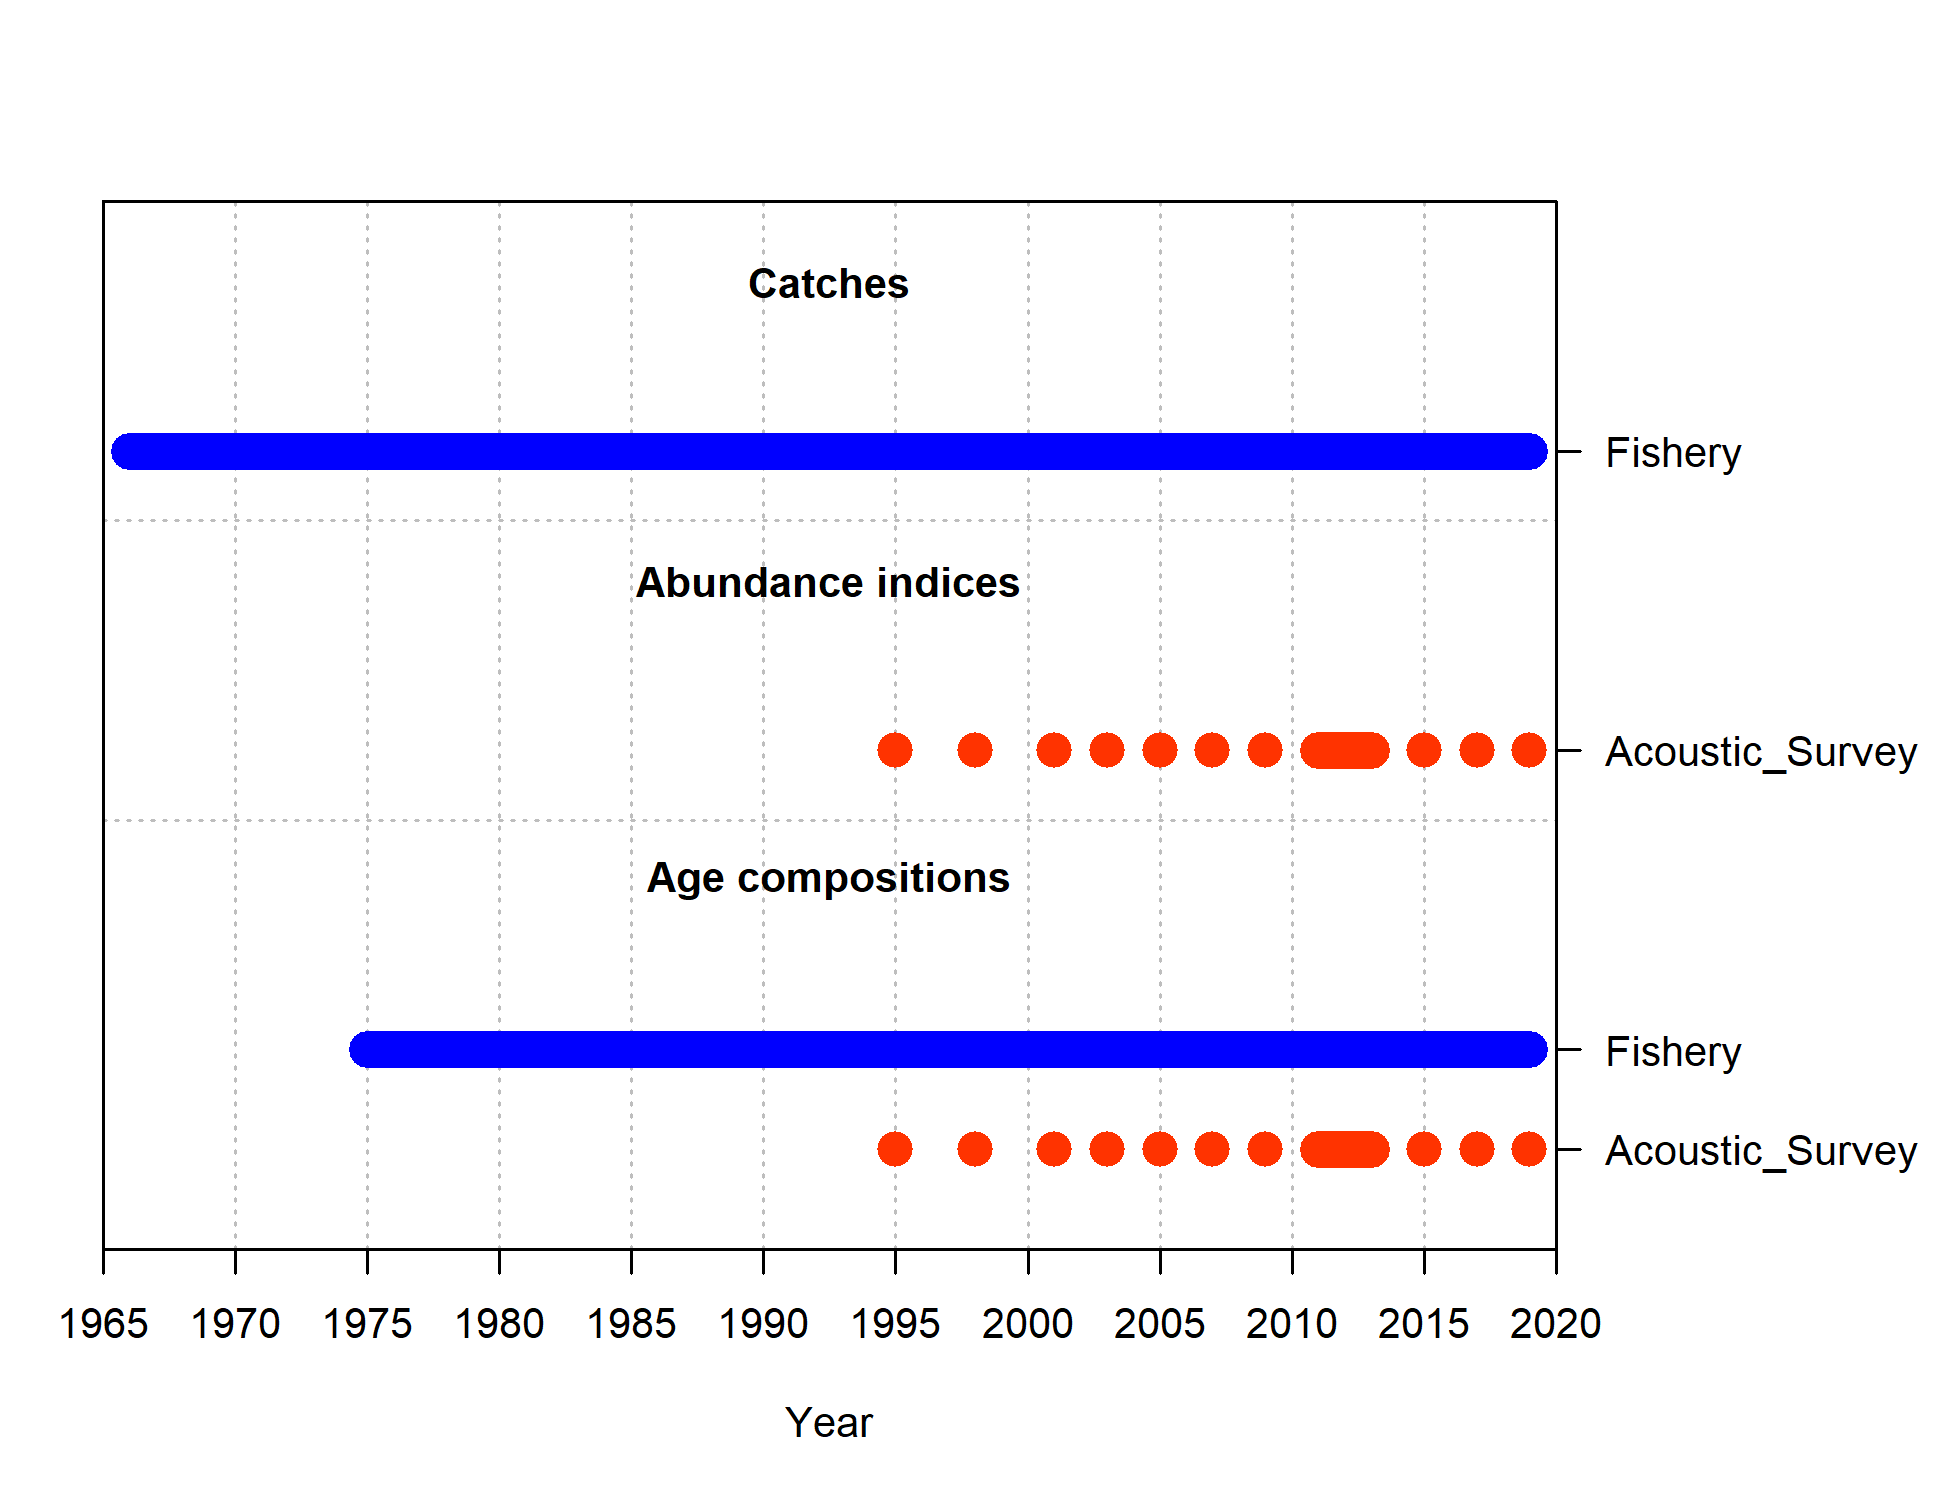
\includegraphics[width=1\textwidth,height=1\textheight]{data-plot.png}
\caption{Summary of data sources used in the base model.\label{fig:data-plot}}
\end{figure}
\end{document}
